\documentclass[acmsmall,review,nonacm]{acmart}\settopmatter{printfolios=true,printccs=false,printacmref=false}

\AtBeginDocument{%
	\providecommand\BibTeX{{%
			\normalfont B\kern-0.5em{\scshape i\kern-0.25em b}\kern-0.8em\TeX}}}

\setcopyright{acmcopyright}
\copyrightyear{2018}
\acmYear{2018}
\acmDOI{10.1145/1122445.1122456}

\usepackage{listings}
\usepackage{lipsum}
\usepackage{xcolor}
\usepackage{multirow}


%% These commands are for a PROCEEDINGS abstract or paper.
\acmConference[Woodstock '18]{Woodstock '18: ACM Symposium on Neural
	Gaze Detection}{June 03--05, 2018}{Woodstock, NY}
\acmBooktitle{Woodstock '18: ACM Symposium on Neural Gaze Detection,
	June 03--05, 2018, Woodstock, NY}
\acmPrice{15.00}
\acmISBN{978-1-4503-XXXX-X/18/06}


\begin{document}
	
	\title{Fine-grained Reductions Around CFL Reachability}
	
	\author{Aleksandra Istomina}
	\thanks{Aleksandra Istomina: graduate student, email: aleksandra2999@mail.ru, ACM student member number: 4678238}
	\email{aleksandra2999@mail.ru}
	\affiliation{%
		\institution{Saint Petersburg State University}
		\city{Saint Petersburg}
		\country{Russia}
	}
	\affiliation{%
	\institution{JetBrains Research}
	\city{Saint Petersburg}
	\country{Russia}
	}

    \author{Research advisor: Semyon Grigorev}
    \affiliation{%
    	\institution{Saint Petersburg State University}
    	\city{Saint Petersburg}
    	\country{Russia}
    }
    \affiliation{%
    	\institution{JetBrains Research}
    	\city{Saint Petersburg}
    	\country{Russia}
    }
	
	\newcommand\todo[1]{{\color{violet}#1}}
	\newcommand\db[1]{{\color{red}#1}}
	\newcommand\question[1]{{\color{cyan}#1}}


	\maketitle
	
	\section{Introduction}
	
	CFL Reachability problem finds application in different fields of research: static code analysis (e.g. type-based flow analysis~\cite{10.1145/373243.360208} or points-to analysis~\cite{10.1145/1103845.1094817, 10.1145/1133255.1134027}), graph databases, bioinformatics. It's goal is to detect valid paths between vertices in a graph. 
	
	There are several cubic~\cite{10.1145/298514.298576, 10.1145/199448.199462} and slightly subcubic~\cite{10.1145/1328438.1328460} (with time $\mathcal{O}(n^{3} / polylog(n))$) algorithms for CFL rechabilty. The big open question is whether a truly subcubic (with time $\tilde{\mathcal{O}}(n^{3 - \epsilon}) = \mathcal{O}(n^{3 - \epsilon} \cdot polylog(n))$) algorithm exists. 
	
	One of the ways to answer that question is given by fine-grained complexity. If one makes a fine-grained reduction from other problem that is known or strongly believed to have some lower bound to CFL Reachability problem, then CFL Reachability problem will also have lower bound. Currently there are several results in the area, but they are scattered and have no structure.
	
	In this paper we give an overview on these existing results: what is already achieved and what questions are still to be answered. We have focused mostly on static problems and connections between them, dynamic problems are omitted from this paper.
	
	\section{Preliminaries}
	
	\emph{Context-free grammar} (CFG) is a four $G=(N, \Sigma, P, S)$, where $N$ is a set of nonterminals, $\Sigma$ is a set of terminals, $P$ is a set of productions of the followings form: $A \to \alpha$, $\alpha \in (N \cup \Sigma)^*$ ans $S$ is a starting nonterminal. Denote a context-free language of words derived from the starting symbol as $L(G)$.
	
	\emph{CFG Recognition} problem is to decide whether $w \in L(G)$ given a CFG $G$ and a string $w \in \Sigma^*$. This problem is closely related to \emph{CFG parsing problem} where we want a possible derivation sequence, if $w \in L(G)$. It is known~\cite{10.5555/646233.682379} that CFG recognition is as hard as CFG parsing up to logarithmic factors.
		
	Let $D = (V, E)$ be a directed graph which edges are labelled with symbols from $P$. We call a path from vertex $v$ to vertex $u$ an $S$-path if concatenation of labels on that path is a word from $L(G)$.  \emph{Context-free-language (CFL) Reachability} problem~\cite{10.1145/258994.259006} is to determine if there exists an $S$-path between a given sets of vertices $A, B$. In \emph{single source/single target (s-t)} CFL Reachability $A = \{s\}, B = \{t\}, s, t \in V(D)$. In \emph{all-pairs} CFL Reachability $A = B = V(D)$.
	
	\emph{Dyck-$k$} reachability problem is a CFL reachability problem where $G$ defines a Dyck language on $k$ types of parentheses. The corresponding grammar is $G=(N, \Sigma, P, S)$, where $N = \{S\}, \Sigma = \{(_i, )_i\}, \forall i = 1, \ldots, k$, productions rules are $S \rightarrow \epsilon | SS | (_1 S )_1 | \ldots | (_k S )_k$, where $\epsilon$ is the empty string. 
	
	For problems $P, Q$ and time bounds $t_P, t_Q$, a \emph{fine-grained reduction}~\cite{bringmann2019fine} from $(P, t_P)$ to $(Q, t_Q)$ is an algorithm that, given an instance $I$ of $P$, computes an instance $J$ of $Q$ such that: 
	
	\begin{itemize}
		\item $I$ is a YES-instance of $P$ if and only if $J$ is a YES-instance of $Q$,
		\item for any $\epsilon > 0$ there is a $\delta > 0$ such that $t_Q(|J|)^{1 - \epsilon} = \mathcal{O}(t_P (|I|)^{1 - \delta})$, 
		\item the running time of the reduction is $\mathcal{O}(t_P (|I|)^{1 - \gamma})$ for some $\gamma > 0$.
	\end{itemize}

	
	\section{Main Results}
	
	This section is organised as follows. Firstly, we define necessary problems. Secondly we present a map of existing fine-grained reductions and make an overview of the most interesting ones. After that we state some open problems and possible ways to solve them. 
	
	\begin{figure}[!htp]
		
		\begin{center}  
			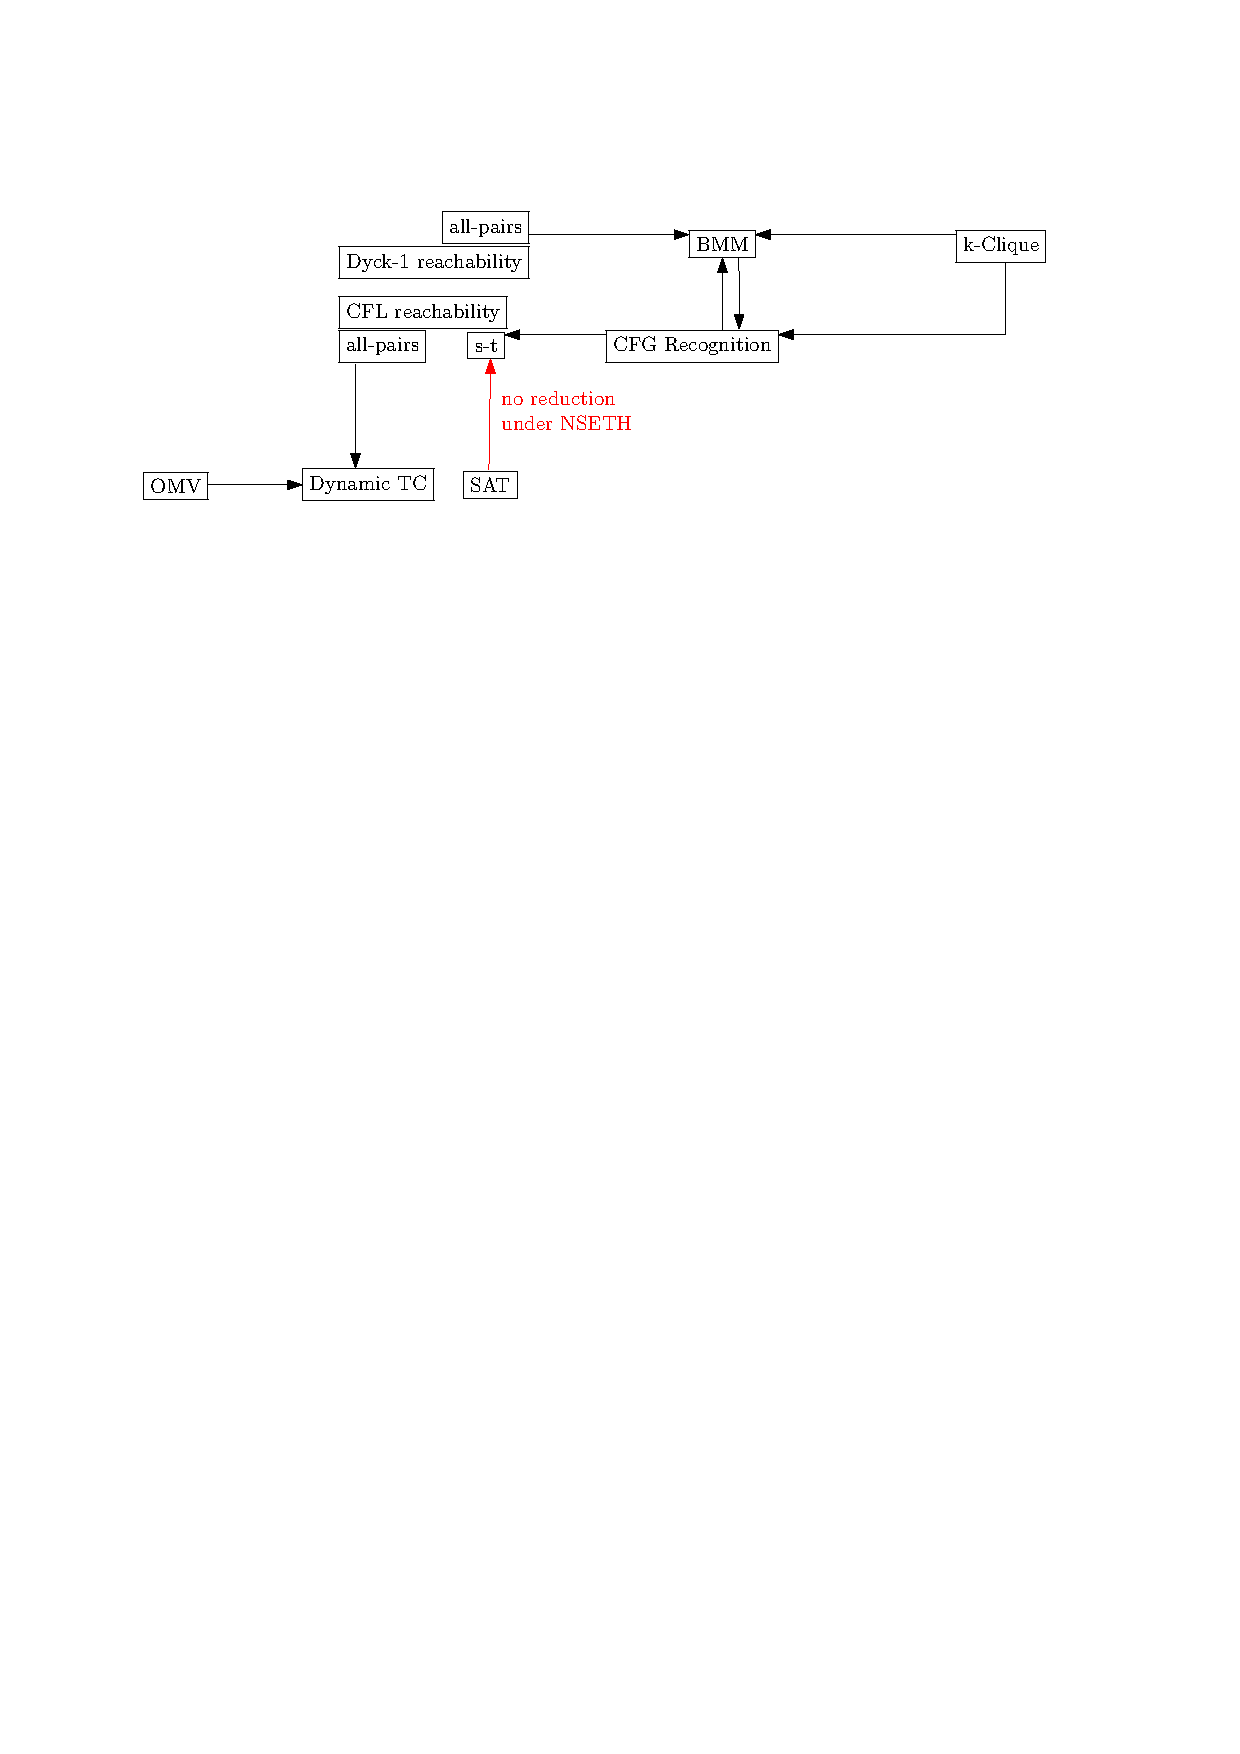
\includegraphics[scale = 0.8]{map_popl.pdf}
		\end{center}
	
		\caption{Existing reductions concerning CFL Reachability and CFG Recognition. Black arrow $a \rightarrow b$ represent existing reduction from $a$ to $b$. Red arrow analogously represent non-existence of the reduction. }
		
	\end{figure}
	
	\subsection{Existing problems and hypotheses}
	
	There are several problems that are connected with CFL Recognition and Reachability. 
	
	\emph{Boolean satisfiability problem (SAT, $k$-SAT)} is to determine if there exists an interpretation of variables that satisfies a given Boolean formula on $n$ variables written in $k$-CNF, $k > 3$. The hypothesis about SAT, that we are interested about, is NSETH~\cite{10.1145/2840728.2840746} which proposes that there is no $\epsilon > 0$ such that $k$-SAT can be solved co-nondeterministically in time $2^{(1 - \epsilon) n}$ for any $k$.
	
	In \emph{Boolean Matrix Multiplication (BMM)} problem it is needed to calculate matrix product of the two given $n \times n$ matrices over (AND, OR). BMM hypothesis states that there is no $\mathcal{O}(n^{3 - \epsilon})$ combinatorial algorithm for that. 
	
	\emph{Orthogonal Vectors (OV)} problem decides whether two sets $X, Y$ of $n$ boolean $d$-dimensional vectors contain a pair $x \in X, y \in Y$ which dot product equals zero. Hypothesis states that OV problem can not be solved in $\mathcal{O}(n^{2 - \epsilon} \cdot poly(d))$ time. 
	
	Given an undirected graph $U$ the \emph{$k$-Clique} problem seeks the clique on $k$ vertices in $U$. 
	
	The incremental \emph{Dynamic Transitive Closure (DTC)}~\cite{Hanauer2020FasterFD} problem asks to maintain reachability information in a directed graph between arbitrary pairs of vertices under insertions of edges.
	
	In the \emph{Online boolean Matrix-Vector multiplication (OMV)}~\cite{10.5555/3039686.3039828} problem we are given an $n \times n$ boolean matrix$M$, we receive $n$ boolean vectors $v_1, \ldots, v_n$ one at a time, and are required to output $Mv_i$ (over the boolean semiring) before seeing the vector $v_{i+1}$, for all $i$.
	
	\subsection{Existing reductions}
	
	Here we present fine-grained complexity results about CFL Reachability and Recognition problems.
	
	First of all we need to mention the interconvertibility of CFL Reachability problems and a class of set-constraint problems~\cite{10.1145/258993.259006} as this result allows us to reformulate our problem if we wish so.
	
	One of the interesting reductions was a reduction from  all-pairs Dyck-1 Reachability problem to BMM problem~\cite{bradford2017efficient},~\cite{10.1145/3434315}. It was firstly proved by Bradford via algebraic matrix encoding and then combinatorially by combining Dyck-1 path from bell-shaped paths.
		
	In one of the recent papers~\cite{inbook} the reduction from all-pairs CFL Reachability to incremental DTC have been proven.
	
	The following results are the most interesting ones concerning the existence of  the truly subcubic algorithm for CFL Reachability.
	
	The problem has been shown to be 2NPDA-complete~\cite{10.5555/788019.788876}. It means that subcubic algorithm for CFL Reachability would lead to subcubic algorithms for the whole 2NPDA class and cubic upper bound has not been improved since discovery of the class in 1968.
	
	Non-existence of the truly subcubic combinatorial algorithm for s-t CFL Reachability under BMM hypothesis was proved combining two reductions: the combinatorial reduction from CFG recognition to s-t CFL reachability~\cite{10.1145/3158118} and combinatorial reduction from BMM to CFG Recogniiton~\cite{10.1145/505241.505242}. This means that if one wants to find the truly subcubic algorithm for CFL Reachability, it should not be combinatorial one.
	
	Recently it was discovered~\cite{chistikov2021subcubic} that there exist subcubic certificates for s-t CFL Reachability (for existence and non-existence of the valid paths). From this fact it follows that there are no reductions under NSETH from SAT problem to CFL Reachability problem.

	\subsection{Open problems}
	
	The equivalence under subcubic reduction of s-t and all-pairs CFL reachability is not yet discovered. However it is known~\cite{10.1145/3186893} that detecting one triangle of a total negative edge weight in a weighted graph and up to $n^{3 - \epsilon}, \epsilon > 0$ such triangles are subcubic equivalent tasks. 
	
	 Currently there is no non-trivial lower bound on Dyck-1 reachability problem. 
	 Yet we know that there exists a reduction from OV problem to Andersen pointer analysis~\cite{10.1145/3434315} where as a part of reduction appears slightly modified Dyck-1 reachability with additional if-condition for edge existence in a graph. If similar reduction exists to pure Dyck-1 reachability problem it would give conditional quadratic lower bound. 
	 
	 Finding a fine-grained reduction from all-pairs shortest paths (APSP) problem or OMV problem to CFL reachability problem would give a conditional lower bound on it's complexity. We highlight APSP problem and it's subcubic equivalent analogues~\cite{10.1145/3186893} as APSP is connected to problems on paths. We highlight OMV problem as it is connected to dynamic problems as is CFL reachability problem. 
	
	\section{Conclusion and Future work}
	
	In this paper we have collected existing results in fine-grained complexity concerning CFL Reachability and CFG Recognition problems. We have presented existing reductions and some open problems with possible ways of their solution. 
	
	CFL reachability is a popular problem strongly connected with many areas. It has several cubic algorithms and no truly subcubic combinatorial one under BMM hypothesis. It has been proved that we can't get cubic lower bound on CFL reachability using reduction from SAT under NSETH. 
	
	Still other reductions may be possible. For example, from APSP or OMV problems. Getting cubic lower bound through them is a possible way of future work as is closing other open problems. 
	
	This overview was focused on static problems and reductions between them. We have reached the DTC problem in a big field of dynamic problems, where are many reductions of our interest. We plan to extend our research there. 
	
	\section{Acknowledgments}
	
	This research was supported by ...
	
	\bibliographystyle{ACM-Reference-Format}
	\bibliography{map}
	
	\appendix
	
\end{document}
\endinput
